\documentclass{beamer}\usepackage{graphicx, color}
%% maxwidth is the original width if it is less than linewidth
%% otherwise use linewidth (to make sure the graphics do not exceed the margin)
\makeatletter


\usetheme{Madrid}
%\hypersetup{pdfpagemode=FullScreen}

\setbeamertemplate{footline}[text line]{} % makes the footer EMPTY
\useoutertheme[subsection=false]{smoothbars}

\usepackage{graphicx}
\usepackage{amsthm}


\begin{document}





\begin{frame}
\LARGE
Version Control and Reproducible Research with GitHub \\
\begin{center}
\vspace{2cm}
Tad Dallas \\
December 2013 \\
\end{center}

\includegraphics[width=0.2\textwidth]{ceesglogo.png}
\hfill 
\includegraphics[width=0.2\textwidth]{github-logo.png}
\end{frame}



\begin{frame}
 \frametitle{What is GitHub?}
``Dropbox on crack''\\
Code sharing, publishing and development service for collaborative projects

\begin{block}{Why use it?}
 \begin{itemize}
  \item Version control 
  \item Open collaboration with other scientists
  \item Creepily watch what other people are working on!
 \end{itemize}
\end{block}


\begin{block}{Under the hood}
 \begin{itemize}
  \item Git is the version control language that GitHub is the GUI for
  \item Created by Linus Torvalds, a central developer of the Linux OS 
  \item Command-line, but really straight-forward
 \end{itemize}
\end{block}
\end{frame}


\begin{frame}
 \frametitle{A couple quick definitions}
  \begin{itemize}
    \item \textbf{Repository}: Storage space where your projects reside
    \item \textbf{Commit}: Takes 'snapshot' of your repository, so you can log a new change, or revert to a previous state (Common command)
    \item \textbf{Branch}: Think of a folder within a repository, but cooler. More on this later
    \item \textbf{Fork}: What it sounds like. You're taking someone's project and making a copy of it for your own use (either to collaborate and to merge later or to use as a template for a different project)
    \item \textbf{Push}: The act of updating your project files (you will ``push'' your \textbf{commits})
    \item \textbf{Pull}: Gets commits from a repository to your machine
    \item \textbf{Fetch}: A better version of \textbf{pull} that doesn't merge \textbf{commits}
  \end{itemize}
  \end{frame}








\begin{frame}
 \frametitle{How to begin}
\begin{enumerate}
 \item Set up an account (go to https://github.com/) and download Git (http://git-scm.com/downloads)
 \item Open a terminal window
\pause
\begin{center}
 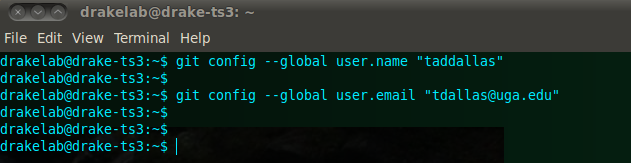
\includegraphics[width=0.85\textwidth]{config.png}
\end{center}
\end{enumerate}
Okay. Now we have Git set up locally. Let's do something with it!

\end{frame}


\begin{frame}
 \frametitle{The GitHub framework}




\end{frame}




\begin{frame}
 \frametitle{\textbf{Make your directory}}

 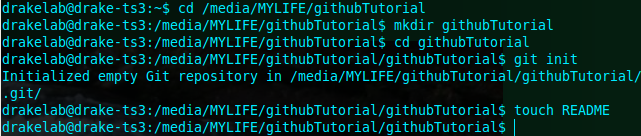
\includegraphics[width=\textwidth]{mkdir.png}\\
\end{frame}

\begin{frame}
\frametitle{\textbf{Commit your README file}}
 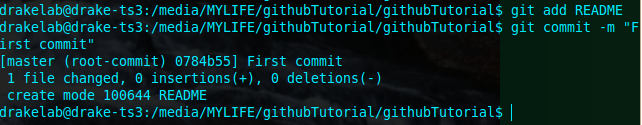
\includegraphics[width=\textwidth]{add.png}\\
\end{frame}

\begin{frame}
\frametitle{\textbf{Push it!}}
 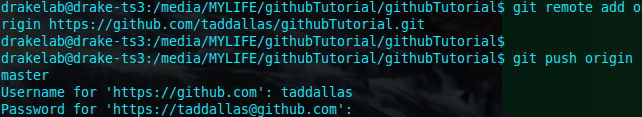
\includegraphics[width=\textwidth]{push.png}\\
\end{frame}


\begin{frame}
 \frametitle{General framework for edits thereafter}
\begin{block}{}
 \begin{enumerate}
  \item Edit your files locally
  \item \$ git add *your files*
  \item \$ git commit -m ``message about this commit''
  \item \$ git push origin master 
 \end{enumerate}
\end{block}
\end{frame}



\begin{frame}
 \frametitle{Forking a repo}

\end{frame}












\end{document}
